% Options for packages loaded elsewhere
\PassOptionsToPackage{unicode}{hyperref}
\PassOptionsToPackage{hyphens}{url}
\documentclass[
]{article}
\usepackage{xcolor}
\usepackage[margin=1in]{geometry}
\usepackage{amsmath,amssymb}
\setcounter{secnumdepth}{-\maxdimen} % remove section numbering
\usepackage{iftex}
\ifPDFTeX
  \usepackage[T1]{fontenc}
  \usepackage[utf8]{inputenc}
  \usepackage{textcomp} % provide euro and other symbols
\else % if luatex or xetex
  \usepackage{unicode-math} % this also loads fontspec
  \defaultfontfeatures{Scale=MatchLowercase}
  \defaultfontfeatures[\rmfamily]{Ligatures=TeX,Scale=1}
\fi
\usepackage{lmodern}
\ifPDFTeX\else
  % xetex/luatex font selection
\fi
% Use upquote if available, for straight quotes in verbatim environments
\IfFileExists{upquote.sty}{\usepackage{upquote}}{}
\IfFileExists{microtype.sty}{% use microtype if available
  \usepackage[]{microtype}
  \UseMicrotypeSet[protrusion]{basicmath} % disable protrusion for tt fonts
}{}
\makeatletter
\@ifundefined{KOMAClassName}{% if non-KOMA class
  \IfFileExists{parskip.sty}{%
    \usepackage{parskip}
  }{% else
    \setlength{\parindent}{0pt}
    \setlength{\parskip}{6pt plus 2pt minus 1pt}}
}{% if KOMA class
  \KOMAoptions{parskip=half}}
\makeatother
\usepackage{color}
\usepackage{fancyvrb}
\newcommand{\VerbBar}{|}
\newcommand{\VERB}{\Verb[commandchars=\\\{\}]}
\DefineVerbatimEnvironment{Highlighting}{Verbatim}{commandchars=\\\{\}}
% Add ',fontsize=\small' for more characters per line
\usepackage{framed}
\definecolor{shadecolor}{RGB}{248,248,248}
\newenvironment{Shaded}{\begin{snugshade}}{\end{snugshade}}
\newcommand{\AlertTok}[1]{\textcolor[rgb]{0.94,0.16,0.16}{#1}}
\newcommand{\AnnotationTok}[1]{\textcolor[rgb]{0.56,0.35,0.01}{\textbf{\textit{#1}}}}
\newcommand{\AttributeTok}[1]{\textcolor[rgb]{0.13,0.29,0.53}{#1}}
\newcommand{\BaseNTok}[1]{\textcolor[rgb]{0.00,0.00,0.81}{#1}}
\newcommand{\BuiltInTok}[1]{#1}
\newcommand{\CharTok}[1]{\textcolor[rgb]{0.31,0.60,0.02}{#1}}
\newcommand{\CommentTok}[1]{\textcolor[rgb]{0.56,0.35,0.01}{\textit{#1}}}
\newcommand{\CommentVarTok}[1]{\textcolor[rgb]{0.56,0.35,0.01}{\textbf{\textit{#1}}}}
\newcommand{\ConstantTok}[1]{\textcolor[rgb]{0.56,0.35,0.01}{#1}}
\newcommand{\ControlFlowTok}[1]{\textcolor[rgb]{0.13,0.29,0.53}{\textbf{#1}}}
\newcommand{\DataTypeTok}[1]{\textcolor[rgb]{0.13,0.29,0.53}{#1}}
\newcommand{\DecValTok}[1]{\textcolor[rgb]{0.00,0.00,0.81}{#1}}
\newcommand{\DocumentationTok}[1]{\textcolor[rgb]{0.56,0.35,0.01}{\textbf{\textit{#1}}}}
\newcommand{\ErrorTok}[1]{\textcolor[rgb]{0.64,0.00,0.00}{\textbf{#1}}}
\newcommand{\ExtensionTok}[1]{#1}
\newcommand{\FloatTok}[1]{\textcolor[rgb]{0.00,0.00,0.81}{#1}}
\newcommand{\FunctionTok}[1]{\textcolor[rgb]{0.13,0.29,0.53}{\textbf{#1}}}
\newcommand{\ImportTok}[1]{#1}
\newcommand{\InformationTok}[1]{\textcolor[rgb]{0.56,0.35,0.01}{\textbf{\textit{#1}}}}
\newcommand{\KeywordTok}[1]{\textcolor[rgb]{0.13,0.29,0.53}{\textbf{#1}}}
\newcommand{\NormalTok}[1]{#1}
\newcommand{\OperatorTok}[1]{\textcolor[rgb]{0.81,0.36,0.00}{\textbf{#1}}}
\newcommand{\OtherTok}[1]{\textcolor[rgb]{0.56,0.35,0.01}{#1}}
\newcommand{\PreprocessorTok}[1]{\textcolor[rgb]{0.56,0.35,0.01}{\textit{#1}}}
\newcommand{\RegionMarkerTok}[1]{#1}
\newcommand{\SpecialCharTok}[1]{\textcolor[rgb]{0.81,0.36,0.00}{\textbf{#1}}}
\newcommand{\SpecialStringTok}[1]{\textcolor[rgb]{0.31,0.60,0.02}{#1}}
\newcommand{\StringTok}[1]{\textcolor[rgb]{0.31,0.60,0.02}{#1}}
\newcommand{\VariableTok}[1]{\textcolor[rgb]{0.00,0.00,0.00}{#1}}
\newcommand{\VerbatimStringTok}[1]{\textcolor[rgb]{0.31,0.60,0.02}{#1}}
\newcommand{\WarningTok}[1]{\textcolor[rgb]{0.56,0.35,0.01}{\textbf{\textit{#1}}}}
\usepackage{graphicx}
\makeatletter
\newsavebox\pandoc@box
\newcommand*\pandocbounded[1]{% scales image to fit in text height/width
  \sbox\pandoc@box{#1}%
  \Gscale@div\@tempa{\textheight}{\dimexpr\ht\pandoc@box+\dp\pandoc@box\relax}%
  \Gscale@div\@tempb{\linewidth}{\wd\pandoc@box}%
  \ifdim\@tempb\p@<\@tempa\p@\let\@tempa\@tempb\fi% select the smaller of both
  \ifdim\@tempa\p@<\p@\scalebox{\@tempa}{\usebox\pandoc@box}%
  \else\usebox{\pandoc@box}%
  \fi%
}
% Set default figure placement to htbp
\def\fps@figure{htbp}
\makeatother
\setlength{\emergencystretch}{3em} % prevent overfull lines
\providecommand{\tightlist}{%
  \setlength{\itemsep}{0pt}\setlength{\parskip}{0pt}}
\usepackage{bookmark}
\IfFileExists{xurl.sty}{\usepackage{xurl}}{} % add URL line breaks if available
\urlstyle{same}
\hypersetup{
  pdftitle={Análisis Estadístico de Datos - Taller 02},
  pdfauthor={Adriana Porras, Alejandra Niño, Bayron Morales, Juliana Cárdenas},
  hidelinks,
  pdfcreator={LaTeX via pandoc}}

\title{Análisis Estadístico de Datos - Taller 02}
\author{Adriana Porras, Alejandra Niño, Bayron Morales, Juliana
Cárdenas}
\date{}

\begin{document}
\maketitle

\subsection{EIA data}\label{eia-data}

U.S. Energy Information Administration (EIA) es una organización que se
encarga de recopilar, analizar y difundir información energética de
manera independiente e imparcial para promover la formulación de
políticas sólidas, mercados eficientes y la comprensión pública de la
energía y su interacción con la economía y el medio ambiente.

Los datos que trabajaremos a continuación corresponden a la extracción
de diferentes variables relacionadas con energías renovables y
combustibles fósiles, las UE son 111 países de todos los continentes del
mundo, seleccionados para fines académicos por ser aquellos países que
presentan mayor cantidad de información de análisis.

El objetivo de este análisis es encontrar diferentes relaciones entre
los países que se están estudiando, de tal forma que podamos
caracterizar en términos de importación, exportación, consumo,
producción, etc. a los países de estudio.

\begin{Shaded}
\begin{Highlighting}[]
\CommentTok{\# Instalación de librerias en caso de no tenerlas}
\CommentTok{\# install.packages("plotly")}
\CommentTok{\# install.packages("MASS")}
\CommentTok{\# install.packages("psych")}
\CommentTok{\# install.packages("tidyverse")}
\CommentTok{\# install.packages("factoextra")}
\CommentTok{\# install.packages("GGally")}

\CommentTok{\# Ejecución de librerias}
\FunctionTok{library}\NormalTok{(plotly)}
\FunctionTok{library}\NormalTok{(MASS)}
\FunctionTok{library}\NormalTok{(psych)}
\FunctionTok{library}\NormalTok{(tidyverse)}
\FunctionTok{library}\NormalTok{(factoextra)}
\FunctionTok{library}\NormalTok{(GGally)}
\end{Highlighting}
\end{Shaded}

\begin{Shaded}
\begin{Highlighting}[]
\CommentTok{\# Colores usados en todos los gráficos del taller}
\NormalTok{rojo        }\OtherTok{\textless{}{-}} \StringTok{"\#DA0921"}
\NormalTok{rojo\_oscuro }\OtherTok{\textless{}{-}} \StringTok{"\#950606"}
\end{Highlighting}
\end{Shaded}

\begin{Shaded}
\begin{Highlighting}[]
\NormalTok{data1 }\OtherTok{\textless{}{-}} \FunctionTok{read.csv}\NormalTok{(}\StringTok{"datos\_taller\_02.csv"}\NormalTok{, }\AttributeTok{row.names=}\DecValTok{1}\NormalTok{, }\AttributeTok{sep=}\StringTok{";"}\NormalTok{)}

\CommentTok{\# Revisar variables en la base}
\FunctionTok{names}\NormalTok{(data1)}
\end{Highlighting}
\end{Shaded}

\begin{verbatim}
##  [1] "Bunker_fuel_consumption_TBPD"                                  
##  [2] "Bunker_residual_fuel_oil_consumption_TBPD"                     
##  [3] "Crude_oil_including_lease_condensate_exports_TBPD"             
##  [4] "Crude_oil_including_lease_condensate_imports_TBPD"             
##  [5] "Crude_oil_including_lease_condensate_production_TBPD"          
##  [6] "Crude_oil_including_lease_condensate_reserves_BB"              
##  [7] "Distillate_fuel_oil_consumption_TBPD"                          
##  [8] "Distillate_fuel_oil_production_TBPD"                           
##  [9] "Jet_fuel_consumption_TBPD"                                     
## [10] "Jet_fuel_production_TBPD"                                      
## [11] "Kerosene_consumption_TBPD"                                     
## [12] "Kerosene_production_TBPD"                                      
## [13] "Liquefied_petroleum_gases_.LPG._consumption_TBPD"              
## [14] "Liquefied_petroleum_gases_.LPG._production_TBPD"               
## [15] "Motor_gasoline_consumption_TBPD"                               
## [16] "Motor_gasoline_production_TBPD"                                
## [17] "Natural_gas_plant_liquids_production_TBPD"                     
## [18] "Other_liquids_production_TBPD"                                 
## [19] "Other_refined_products_consumption_TBPD"                       
## [20] "Other_refined_products_production_TBPD"                        
## [21] "Petroleum_and_other_liquids_CO2_emissions_MMTCD"               
## [22] "Petroleum_and_other_liquids_consumption_TBPD"                  
## [23] "Petroleum_and_other_liquids_production_TBPD"                   
## [24] "Refined_petroleum_products_consumption_TBPD"                   
## [25] "Refined_petroleum_products_production_TBPD"                    
## [26] "Refinery_processing_gain_TBPD"                                 
## [27] "Residual_fuel_oil_consumption_TBPD"                            
## [28] "Residual_fuel_oil_production_TBPD"                             
## [29] "Biomass_and_waste_electricity_installed_capacity_MK"           
## [30] "Biomass_and_waste_electricity_net_generation_BKWH"             
## [31] "Electricity_distribution_losses_BKWH"                          
## [32] "Electricity_exports_BKWH"                                      
## [33] "Electricity_imports_BKWH"                                      
## [34] "Electricity_installed_capacity_MK"                             
## [35] "Electricity_net_consumption_BKWH"                              
## [36] "Electricity_net_generation_BKWH"                               
## [37] "Electricity_net_imports_BKWH"                                  
## [38] "Fossil_fuels_electricity_installed_capacity_MK"                
## [39] "Fossil_fuels_electricity_net_generation_BKWH"                  
## [40] "Geothermal_electricity_installed_capacity_MK"                  
## [41] "Geothermal_electricity_net_generation_BKWH"                    
## [42] "Hydroelectric_pumped_storage_electricity_installed_capacity_MK"
## [43] "Hydroelectric_pumped_storage_electricity_net_generation_BKWH"  
## [44] "Hydroelectricity_installed_capacity_MK"                        
## [45] "Hydroelectricity_net_generation_BKWH"                          
## [46] "Non.hydro_renewable_electricity_installed_capacity_MK"         
## [47] "Non.hydro_renewable_electricity_net_generation_BKWH"           
## [48] "Nuclear_electricity_installed_capacity_MK"                     
## [49] "Nuclear_electricity_net_generation_BKWH"                       
## [50] "Renewable_electricity_installed_capacity_MK"                   
## [51] "Renewable_electricity_net_generation_BKWH"                     
## [52] "Solar_electricity_installed_capacity_MK"                       
## [53] "Solar_electricity_net_generation_BKWH"                         
## [54] "Tide_and_wave_electricity_installed_capacity_MK"               
## [55] "Tide_and_wave_electricity_net_generation_BKWH"                 
## [56] "Wind_electricity_installed_capacity_MK"                        
## [57] "Wind_electricity_net_generation_BKWH"
\end{verbatim}

\begin{center}\rule{0.5\linewidth}{0.5pt}\end{center}

\subsection{Normal multivariada}\label{normal-multivariada}

\noindent\textbf{Pregunta 1. Encuentre la estimación del vector de medias y la matriz de varianzas y covarianzas para 5 variables de su interés del conjunto de datos.}

Las 5 variables seleccionadas son:

\begin{itemize}
\item
  Electricity\_net\_consumption\_BKWH (35)
\item
  Electricity\_net\_generation\_BKWH (36)
\item
  Electricity\_distribution\_losses\_BKWH (31)
\item
  Fossil\_fuels\_electricity\_net\_generation\_BKWH (39)
\item
  Renewable\_electricity\_net\_generation\_BKWH (51)
\end{itemize}

\begin{Shaded}
\begin{Highlighting}[]
\NormalTok{data2 }\OtherTok{\textless{}{-}}\NormalTok{ data1[}\FunctionTok{c}\NormalTok{(}\DecValTok{35}\SpecialCharTok{:}\DecValTok{36}\NormalTok{,}\DecValTok{31}\NormalTok{,}\DecValTok{39}\NormalTok{,}\DecValTok{51}\NormalTok{)]}

\CommentTok{\# Se ajustan los nombres para facilitar la visualización}
\FunctionTok{names}\NormalTok{(data2) }\OtherTok{\textless{}{-}} \FunctionTok{c}\NormalTok{(}\StringTok{"Consumo(C)"}\NormalTok{, }\StringTok{"Generacion(G)"}\NormalTok{,}\StringTok{"Perdida(P)"}\NormalTok{,}
                  \StringTok{"Fossil\_G"}\NormalTok{, }\StringTok{"Renewable\_G"}\NormalTok{)}

\FunctionTok{names}\NormalTok{(data2)}
\end{Highlighting}
\end{Shaded}

\begin{verbatim}
## [1] "Consumo(C)"    "Generacion(G)" "Perdida(P)"    "Fossil_G"     
## [5] "Renewable_G"
\end{verbatim}

\begin{Shaded}
\begin{Highlighting}[]
\CommentTok{\# Vector de medias}
\FunctionTok{colMeans}\NormalTok{(data2)}
\end{Highlighting}
\end{Shaded}

\begin{verbatim}
##    Consumo(C) Generacion(G)    Perdida(P)      Fossil_G   Renewable_G 
##     181.81592     198.29009      17.00450     132.58408      44.77117
\end{verbatim}

Es necesario resaltar que las cinco variables seleccionadas manejan la
misma escala, ya que se presentan en BKWH (Billion Kilowatt Hours (Miles
de millones de kilovatios-hora)). Respecto al vector de medias, la
generación neta de electricidad es la que tiene la mayor media
(Generación(G): 198.290 BKWH), seguido por el consumo neto de
electricidad (Consumo(C): 181.816 BKWH) y la generación neta de
electricidad a partir de combustibles fósiles (Fossil\_G: 132.584). La
generación neta de electricidad renovable tiene una media de 44,771 y la
media más baja la tienen las pérdidas en la distribución de
electricidad. Esta última variable representa la diferencia entre la
energía eléctrica que se inyecta en la red de distribución y la energia
que finalmente se entrega a los consumidores finales.

\begin{Shaded}
\begin{Highlighting}[]
\CommentTok{\# Matriz de varianzas y covarianzas:}
\FunctionTok{cov}\NormalTok{(data2)}
\end{Highlighting}
\end{Shaded}

\begin{verbatim}
##               Consumo(C) Generacion(G) Perdida(P)  Fossil_G Renewable_G
## Consumo(C)     383958.82     408034.46  25162.312 290441.49   82086.952
## Generacion(G)  408034.46     434094.97  27076.711 308733.29   87623.857
## Perdida(P)      25162.31      27076.71   1990.936  19210.37    5578.751
## Fossil_G       290441.49     308733.29  19210.368 223824.71   60829.937
## Renewable_G     82086.95      87623.86   5578.751  60829.94   20864.464
\end{verbatim}

La variable que presenta mayor varianza es consumo neto de electricidad
(Consumo(C): 383958) y la que presenta menor varianza es pérdidas en la
distribución de electricidad (Perdida(P): 1990.936). Sin embargo, se
debe recordar que esta se ve afectada por valores atípicos, por lo que
puede estar sobrestimada.

Respecto a las covarianza, se observa que todas las variables se
relacionan positivamente, es decir, que al aumentar una, las otras
también aumentarán. Para poder medir la fuerza de esa relación, se
requiere realizar un análisis de correlación, el cual se realizará en el
siguiente punto.

\begin{center}\rule{0.5\linewidth}{0.5pt}\end{center}

\subsection{ACP}\label{acp}

\noindent\textbf{Pregunta 2. Realice un análisis descriptivo univariado y bivariado del conjunto de datos. Considere nuevamente las mismas 5 variables de su interés para este punto.}

\textbf{Análisis descriptivo univariado}

Para realizar el análisis descriptivo univariado se van a emplear
boxplot, por lo que se genera una función que permita realizarlo de
forma fácil y, a continuación, se generan y analizan cada uno de los
boxplot.

\begin{Shaded}
\begin{Highlighting}[]
\CommentTok{\# Crear una función para crear boxplot}

\NormalTok{boxplot\_estadisticos }\OtherTok{\textless{}{-}} \ControlFlowTok{function}\NormalTok{(data2, variable, titulo, subtitulo, etiqueta\_x) \{}
  
\NormalTok{  valores }\OtherTok{\textless{}{-}}\NormalTok{ data2[[variable]]}
  
\NormalTok{  estadisticos }\OtherTok{\textless{}{-}} \FunctionTok{boxplot.stats}\NormalTok{(valores)}\SpecialCharTok{$}\NormalTok{stats}
  
\NormalTok{  etiquetas }\OtherTok{\textless{}{-}} \FunctionTok{data.frame}\NormalTok{(}
    \AttributeTok{x =} \FunctionTok{as.numeric}\NormalTok{(estadisticos),}
    \AttributeTok{y =} \FloatTok{1.18}\NormalTok{,}
    \AttributeTok{etiqueta =} \FunctionTok{c}\NormalTok{(}
      \FunctionTok{paste0}\NormalTok{(}\StringTok{"Mín: "}\NormalTok{, }\FunctionTok{round}\NormalTok{(estadisticos[}\DecValTok{1}\NormalTok{], }\DecValTok{1}\NormalTok{)),}
      \FunctionTok{paste0}\NormalTok{(}\StringTok{"Q1: "}\NormalTok{, }\FunctionTok{round}\NormalTok{(estadisticos[}\DecValTok{2}\NormalTok{], }\DecValTok{1}\NormalTok{)),}
      \FunctionTok{paste0}\NormalTok{(}\StringTok{"Q2: "}\NormalTok{, }\FunctionTok{round}\NormalTok{(estadisticos[}\DecValTok{3}\NormalTok{], }\DecValTok{1}\NormalTok{)),}
      \FunctionTok{paste0}\NormalTok{(}\StringTok{"Q3: "}\NormalTok{, }\FunctionTok{round}\NormalTok{(estadisticos[}\DecValTok{4}\NormalTok{], }\DecValTok{1}\NormalTok{)),}
      \FunctionTok{paste0}\NormalTok{(}\StringTok{"Máx: "}\NormalTok{, }\FunctionTok{round}\NormalTok{(estadisticos[}\DecValTok{5}\NormalTok{], }\DecValTok{1}\NormalTok{))))}
  
  \FunctionTok{ggplot}\NormalTok{(data2, }\FunctionTok{aes}\NormalTok{(}\AttributeTok{x =}\NormalTok{ .data[[variable]], }\AttributeTok{y =} \DecValTok{1}\NormalTok{)) }\SpecialCharTok{+}
    
    \FunctionTok{geom\_boxplot}\NormalTok{(}
      \AttributeTok{fill =}\NormalTok{ rojo,}
      \AttributeTok{color =}\NormalTok{ rojo\_oscuro,}
      \AttributeTok{width =} \FloatTok{0.35}\NormalTok{) }\SpecialCharTok{+}
    
    \FunctionTok{geom\_segment}\NormalTok{(}
      \AttributeTok{data =}\NormalTok{ etiquetas,}
      \FunctionTok{aes}\NormalTok{(}
        \AttributeTok{x =}\NormalTok{ x,}
        \AttributeTok{xend =}\NormalTok{ x,}
        \AttributeTok{y =} \FloatTok{0.82}\NormalTok{,}
        \AttributeTok{yend =} \FloatTok{1.18}
\NormalTok{      ),}
      \AttributeTok{color =}\NormalTok{ rojo\_oscuro,}
      \AttributeTok{linewidth =} \FloatTok{0.5}\NormalTok{,}
      \AttributeTok{linetype =} \StringTok{"dashed"}\NormalTok{) }\SpecialCharTok{+}
    
    \FunctionTok{geom\_text}\NormalTok{(}
      \AttributeTok{data =}\NormalTok{ etiquetas,}
      \FunctionTok{aes}\NormalTok{(}
        \AttributeTok{x =}\NormalTok{ x,}
        \AttributeTok{y =}\NormalTok{ y,}
        \AttributeTok{label =}\NormalTok{ etiqueta}
\NormalTok{      ),}
      \AttributeTok{size =} \FloatTok{3.5}\NormalTok{,}
      \AttributeTok{fontface =} \StringTok{"bold"}\NormalTok{,}
      \AttributeTok{color =} \StringTok{"\#950606"}\NormalTok{) }\SpecialCharTok{+}
    
    \FunctionTok{labs}\NormalTok{(}
      \AttributeTok{title =}\NormalTok{ titulo,}
      \AttributeTok{subtitle =}\NormalTok{ subtitulo,}
      \AttributeTok{x =}\NormalTok{ etiqueta\_x,}
      \AttributeTok{y =} \ConstantTok{NULL}\NormalTok{) }\SpecialCharTok{+}
    
    \FunctionTok{theme\_minimal}\NormalTok{() }\SpecialCharTok{+}
    
    \FunctionTok{theme}\NormalTok{(}
      \AttributeTok{plot.title =} \FunctionTok{element\_text}\NormalTok{(}
        \AttributeTok{face =} \StringTok{"bold"}\NormalTok{,}
        \AttributeTok{size =} \DecValTok{14}\NormalTok{,}
        \AttributeTok{hjust =} \FloatTok{0.5}\NormalTok{),}
      \AttributeTok{plot.subtitle =} \FunctionTok{element\_text}\NormalTok{(}
        \AttributeTok{size =} \DecValTok{11}\NormalTok{,}
        \AttributeTok{hjust =} \FloatTok{0.5}\NormalTok{),}
      \AttributeTok{axis.text.y =} \FunctionTok{element\_blank}\NormalTok{(),}
      \AttributeTok{axis.ticks.y =} \FunctionTok{element\_blank}\NormalTok{(),}
      \AttributeTok{axis.title.y =} \FunctionTok{element\_blank}\NormalTok{(),}
      \AttributeTok{axis.title.x =} \FunctionTok{element\_text}\NormalTok{(}\AttributeTok{face =} \StringTok{"bold"}\NormalTok{),}
      \AttributeTok{panel.grid.minor =} \FunctionTok{element\_blank}\NormalTok{(),}
      \AttributeTok{panel.grid.major.y =} \FunctionTok{element\_blank}\NormalTok{())\}}
\end{Highlighting}
\end{Shaded}

\begin{Shaded}
\begin{Highlighting}[]
\FunctionTok{boxplot\_estadisticos}\NormalTok{(}
\NormalTok{ data2,}
  \StringTok{"Consumo(C)"}\NormalTok{,}
  \StringTok{"Distribución Consumo(C)"}\NormalTok{,}
  \StringTok{"Paises"}\NormalTok{,}
  \StringTok{"Electricidad consumidad(BKWH)"}\NormalTok{)}
\end{Highlighting}
\end{Shaded}

\begin{center}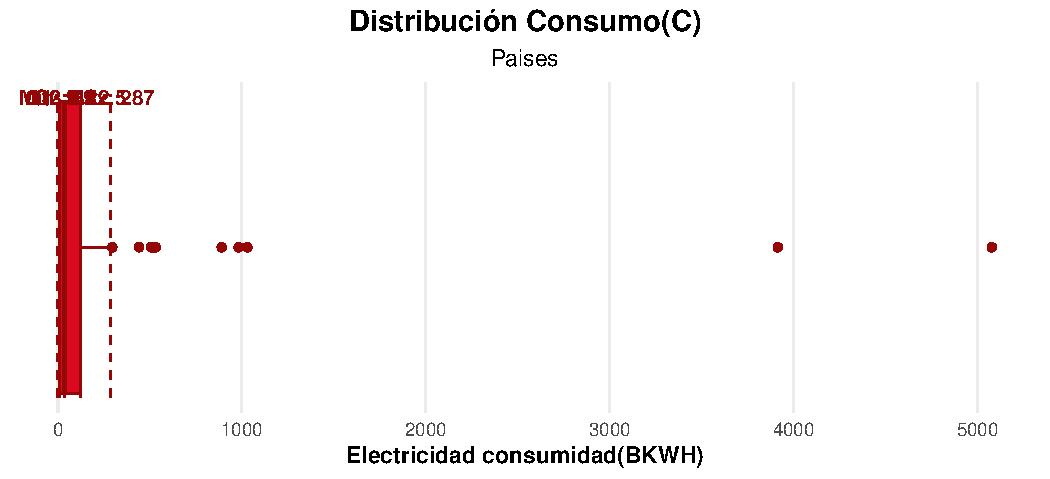
\includegraphics{Taller-02_files/figure-latex/Boxplot Consumo-1} \end{center}

\begin{Shaded}
\begin{Highlighting}[]
\NormalTok{caja\_Consumo }\OtherTok{\textless{}{-}} \FunctionTok{boxplot}\NormalTok{(data2}\SpecialCharTok{$}\StringTok{\textasciigrave{}}\AttributeTok{Consumo(C)}\StringTok{\textasciigrave{}}\NormalTok{, }\AttributeTok{plot =} \ConstantTok{TRUE}\NormalTok{)}
\end{Highlighting}
\end{Shaded}

\begin{center}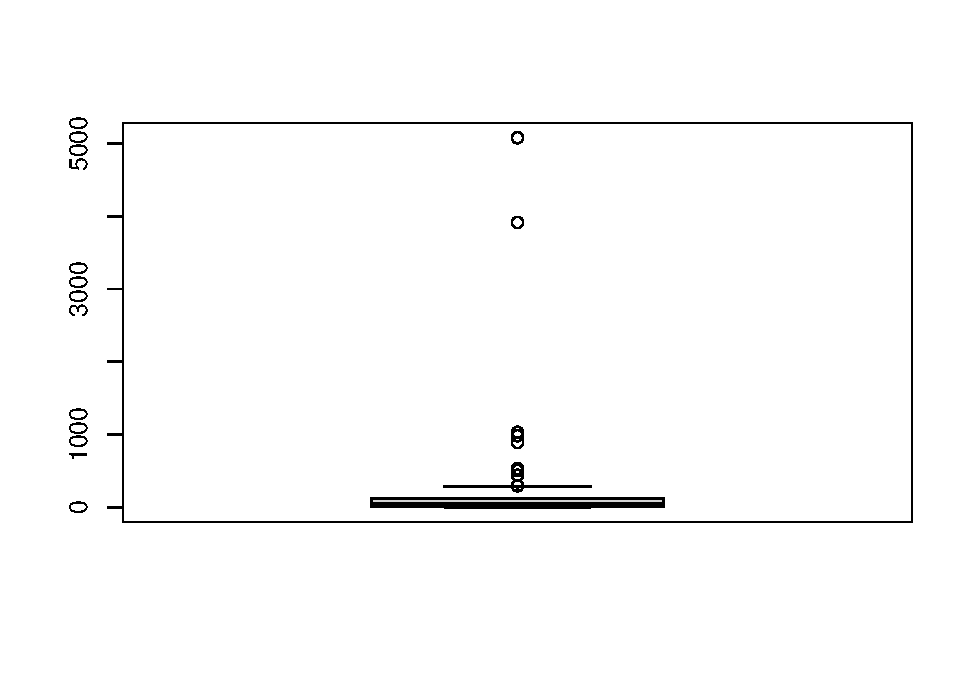
\includegraphics{Taller-02_files/figure-latex/unnamed-chunk-2-1} \end{center}

\begin{Shaded}
\begin{Highlighting}[]
\NormalTok{caja\_Consumo}\SpecialCharTok{$}\NormalTok{stats}
\end{Highlighting}
\end{Shaded}

\begin{verbatim}
##        [,1]
## [1,]   0.80
## [2,]   9.95
## [3,]  37.00
## [4,] 122.50
## [5,] 287.00
\end{verbatim}

\begin{Shaded}
\begin{Highlighting}[]
\FunctionTok{length}\NormalTok{(caja\_Consumo}\SpecialCharTok{$}\NormalTok{out)}
\end{Highlighting}
\end{Shaded}

\begin{verbatim}
## [1] 11
\end{verbatim}

\begin{Shaded}
\begin{Highlighting}[]
\FunctionTok{max}\NormalTok{(data2}\SpecialCharTok{$}\StringTok{\textasciigrave{}}\AttributeTok{Consumo(C)}\StringTok{\textasciigrave{}}\NormalTok{)}
\end{Highlighting}
\end{Shaded}

\begin{verbatim}
## [1] 5079
\end{verbatim}

En el punto anterior se identificó que la media de la generación neta de
electricidad es de 198.290 BKWH, este valor dista bastante de la mediana
(Q2): 37, debido a que la media es sensible a valores atípicos y, en
este caso, se observan 11 datos atipicos con valores muy extremos.

\begin{Shaded}
\begin{Highlighting}[]
\FunctionTok{boxplot\_estadisticos}\NormalTok{(}
\NormalTok{ data2,}
  \StringTok{"Generacion(G)"}\NormalTok{,}
  \StringTok{"Distribución Generacion(G)"}\NormalTok{,}
  \StringTok{"Paises"}\NormalTok{,}
  \StringTok{"Electricidad generada (BKWH)"}\NormalTok{)}
\end{Highlighting}
\end{Shaded}

\begin{center}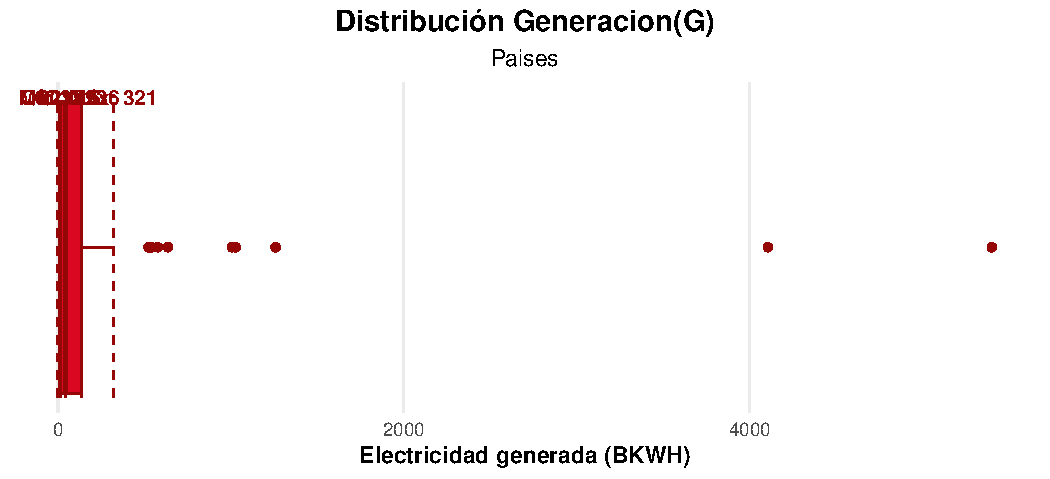
\includegraphics{Taller-02_files/figure-latex/Boxplot generación-1} \end{center}

\begin{Shaded}
\begin{Highlighting}[]
\NormalTok{caja\_Generacion }\OtherTok{\textless{}{-}} \FunctionTok{boxplot}\NormalTok{(data2}\SpecialCharTok{$}\StringTok{\textasciigrave{}}\AttributeTok{Generacion(G)}\StringTok{\textasciigrave{}}\NormalTok{, }\AttributeTok{plot =} \ConstantTok{FALSE}\NormalTok{)}

\NormalTok{caja\_Generacion}\SpecialCharTok{$}\NormalTok{stats}
\end{Highlighting}
\end{Shaded}

\begin{verbatim}
##       [,1]
## [1,]   0.9
## [2,]  12.5
## [3,]  43.0
## [4,] 136.0
## [5,] 321.0
\end{verbatim}

\begin{Shaded}
\begin{Highlighting}[]
\FunctionTok{length}\NormalTok{(caja\_Generacion}\SpecialCharTok{$}\NormalTok{out)}
\end{Highlighting}
\end{Shaded}

\begin{verbatim}
## [1] 9
\end{verbatim}

\ldots..

\begin{Shaded}
\begin{Highlighting}[]
\FunctionTok{boxplot\_estadisticos}\NormalTok{(}
\NormalTok{ data2,}
  \StringTok{"Perdida(P)"}\NormalTok{,}
  \StringTok{"Distribución Perdida(P)"}\NormalTok{,}
  \StringTok{"Paises"}\NormalTok{,}
  \StringTok{"Electricidad consumidad(BKWH)"}\NormalTok{)}
\end{Highlighting}
\end{Shaded}

\begin{center}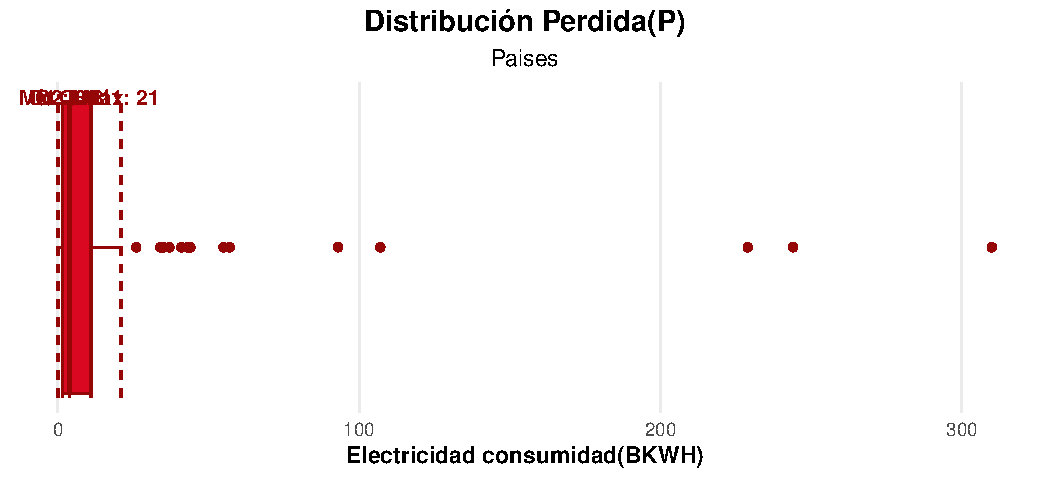
\includegraphics{Taller-02_files/figure-latex/Boxplot Perdida-1} \end{center}

\begin{Shaded}
\begin{Highlighting}[]
\NormalTok{caja\_Perdida }\OtherTok{\textless{}{-}} \FunctionTok{boxplot}\NormalTok{(data2}\SpecialCharTok{$}\StringTok{\textasciigrave{}}\AttributeTok{Perdida(P)}\StringTok{\textasciigrave{}}\NormalTok{, }\AttributeTok{plot =} \ConstantTok{FALSE}\NormalTok{)}

\NormalTok{caja\_Perdida}\SpecialCharTok{$}\NormalTok{stats}
\end{Highlighting}
\end{Shaded}

\begin{verbatim}
##       [,1]
## [1,]  0.10
## [2,]  1.65
## [3,]  3.80
## [4,] 11.00
## [5,] 21.00
\end{verbatim}

\begin{Shaded}
\begin{Highlighting}[]
\FunctionTok{length}\NormalTok{(caja\_Perdida}\SpecialCharTok{$}\NormalTok{out)}
\end{Highlighting}
\end{Shaded}

\begin{verbatim}
## [1] 15
\end{verbatim}

\ldots..

\begin{Shaded}
\begin{Highlighting}[]
\FunctionTok{boxplot\_estadisticos}\NormalTok{(}
\NormalTok{ data2,}
  \StringTok{"Renewable\_G"}\NormalTok{,}
  \StringTok{"Distribución Renewable\_G"}\NormalTok{,}
  \StringTok{"Paises"}\NormalTok{,}
  \StringTok{"Electricidad Renovable (BKWH)"}\NormalTok{)}
\end{Highlighting}
\end{Shaded}

\begin{center}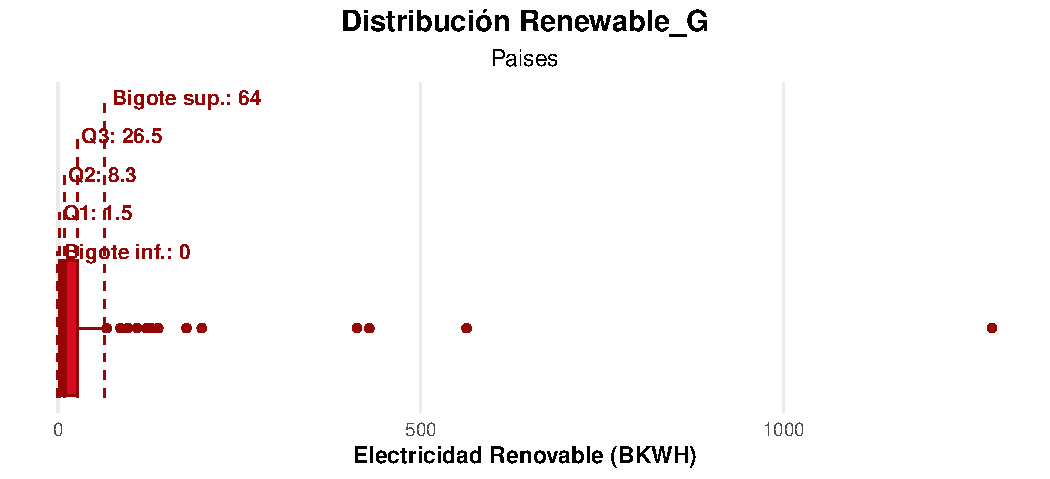
\includegraphics{Taller-02_files/figure-latex/Boxplot Renovable-1} \end{center}

\begin{Shaded}
\begin{Highlighting}[]
\NormalTok{caja\_Renewable\_G }\OtherTok{\textless{}{-}} \FunctionTok{boxplot}\NormalTok{(data2}\SpecialCharTok{$}\NormalTok{Renewable\_G, }\AttributeTok{plot =} \ConstantTok{FALSE}\NormalTok{)}

\NormalTok{caja\_Renewable\_G}\SpecialCharTok{$}\NormalTok{stats}
\end{Highlighting}
\end{Shaded}

\begin{verbatim}
##      [,1]
## [1,]  0.0
## [2,]  1.5
## [3,]  8.3
## [4,] 26.5
## [5,] 64.0
\end{verbatim}

\begin{Shaded}
\begin{Highlighting}[]
\FunctionTok{length}\NormalTok{(caja\_Renewable\_G}\SpecialCharTok{$}\NormalTok{out)}
\end{Highlighting}
\end{Shaded}

\begin{verbatim}
## [1] 13
\end{verbatim}

\ldots..

\begin{Shaded}
\begin{Highlighting}[]
\FunctionTok{gather}\NormalTok{(data2) }\SpecialCharTok{\%\textgreater{}\%}
  \FunctionTok{ggplot}\NormalTok{(}\FunctionTok{aes}\NormalTok{(}\AttributeTok{x=}\NormalTok{value)) }\SpecialCharTok{+}
  \FunctionTok{geom\_density}\NormalTok{() }\SpecialCharTok{+}
  \FunctionTok{labs}\NormalTok{(}\AttributeTok{x=} \StringTok{""}\NormalTok{,}\AttributeTok{y=}\StringTok{\textquotesingle{}Densidad\textquotesingle{}}\NormalTok{,}\AttributeTok{title=}\StringTok{"Densidad estimada"}\NormalTok{) }\SpecialCharTok{+}
  \FunctionTok{facet\_wrap}\NormalTok{(}\SpecialCharTok{\textasciitilde{}}\NormalTok{key, }\AttributeTok{scales =} \StringTok{"free"}\NormalTok{)}
\end{Highlighting}
\end{Shaded}

\begin{center}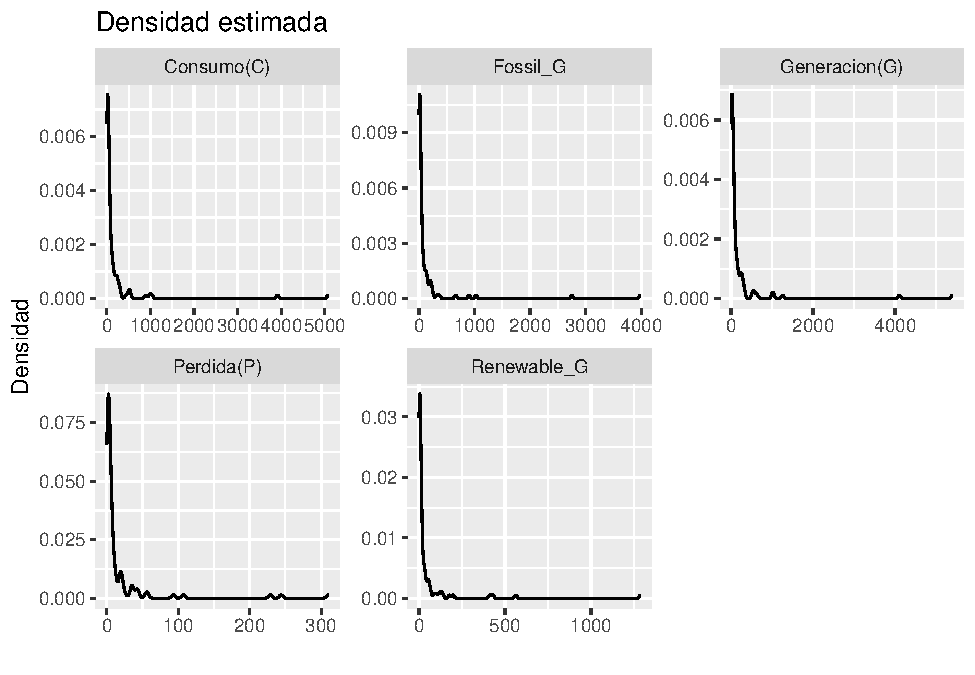
\includegraphics{Taller-02_files/figure-latex/densidad_estimada-1} \end{center}

\textbf{Análisis descriptivo multivariado}

\ldots..

\begin{Shaded}
\begin{Highlighting}[]
\FunctionTok{pairs.panels}\NormalTok{(data2,}
             \AttributeTok{scale =} \ConstantTok{FALSE}\NormalTok{,      }\CommentTok{\# If TRUE, scales the correlation text font}
             \AttributeTok{density =} \ConstantTok{TRUE}\NormalTok{,     }\CommentTok{\# If TRUE, adds density plots and histograms}
             \AttributeTok{method =} \StringTok{"pearson"}\NormalTok{, }\CommentTok{\# Correlation method (also "spearman" or "kendall")}
             \AttributeTok{cor =} \ConstantTok{TRUE}\NormalTok{,         }\CommentTok{\# If TRUE, reports correlations}
             \AttributeTok{jiggle =} \ConstantTok{FALSE}\NormalTok{)     }\CommentTok{\# If TRUE, data points are jittered}
\end{Highlighting}
\end{Shaded}

\begin{center}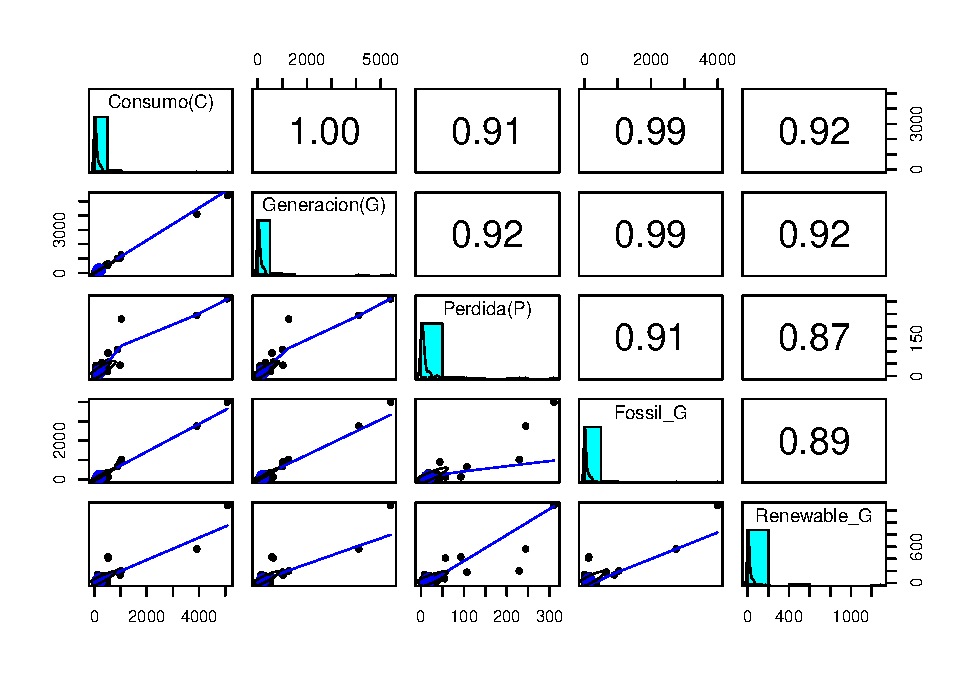
\includegraphics{Taller-02_files/figure-latex/unnamed-chunk-7-1} \end{center}

\ldots..

\noindent\textbf{Pregunta 3. El conjunto de datos incluye 57 variables, analizarlas de forma individual podría representar un gasto computacional y de tiempo bastante agotador; por lo cuál una técnica de reducción de dimensionalidad sería ideal. Ejecute un ACP sobre estos datos, compare la contribución de las variables sobre el primer plano factorial de un ACP normado (escalado) y uno sin normalizar (sin escalar).}

\noindent\textbf{Pregunta 4. Una vez calculado el PCA normado, ¿qué número de componentes principales deberíamos seleccionar? ¿Bajo que criterio seleccionó este número de componentes?}

\noindent\textbf{Pregunta 5. Analice la representación de las variables originales sobre las dos primeras componentes en el primer plano factorial. ¿Que conclusiones podemos sacar de este análisis?}

\noindent\textbf{Pregunta 6. Ahora examine con detenimiento el mapa de individuos sobre los planos factoriales que conforman las componentes (1,2) y (2,3). ¿Qué conclusiones puede sacar según la cercanía de algunas UE?}

\noindent\textbf{Pregunta 7. Como hemos observado en clase, el ACP es una técnica bastante sensible a datos atípicos, ejecute nuevamente el ACP retirando del conjunto de datos a Estados Unidos, China, Arabia Saudi y Rusia. ¿En que cambia el ACP al excluir estos países?. ¿Se perciben clusters de países con mayor claridad?. Calcule únicamente el ACP normado.}

\begin{center}\rule{0.5\linewidth}{0.5pt}\end{center}

\subsection{Clustering}\label{clustering}

\noindent\textbf{Pregunta 8. De acuerdo a lo aprendido en la clase de agrupamiento, utilice el primer plano factorial para determinar de manera aproximada el número de grupos en el análisis. ¿Cuántos clusters espera que existan en el conjunto de datos?}

\noindent\textbf{Pregunta 9. Mediante el método de reducción de varianza explicada, determine un número fijo de clusters para su análisis. No tiene que ser el mismo número que el elegido por su compañero, recuerde que ninguno conoce las etiquetas reales de los grupos de los países.}

\noindent\textbf{Pregunta 10. Determine mediante k-means y aglomeración jerárquica (usando enlace promedio) la clasificación en grupos para los países de estudio. Considere todas las variables de estudio ¿son diferentes los resultados de los dos análisis cluster?}

\noindent\textbf{Pregunta 11. Grafique mediante boxplot la distribución de las 5 variables seleccionadas en el punto 2 diferenciando por los grupos encontrados mediante k-means (es decir, obtenga un boxplot por variable y por grupo: si por ejemplo k-means indica un total de 3 grupos, realice 3 boxplots, uno por grupo, para cada una de las 5 variables). ¿Observa diferencias importantes entre las distribuciones por grupos de la misma variable?}

\end{document}
